\documentclass{article}
\usepackage[T1]{fontenc}
\usepackage{lmodern}
\usepackage{graphicx}
\usepackage{amsmath,amssymb}
\usepackage[a4paper,margin=2cm]{geometry}
\usepackage[absolute,overlay]{textpos}
\setlength{\TPHorizModule}{1mm}
\setlength{\TPVertModule}{1mm}
\usepackage[indonesian]{babel}
\usepackage{hyperref}
\setlength{\emergencystretch}{2em}
% unit: Halaman 42

\begin{document}

% === Halaman 42 (llm) ===

\vspace{139.59mm}

Diagram Blok RC4:\vspace{60mm}
\begin{itemize}
    \item Kunci rahasia (\textit{secret key}) memiliki panjang maksimal 256 karakter (1 karakter = 1byte). Jika panjang kunci kurang dari 256 \textit{byte} maka karakter-karakter kunci diulang secara periodik.
    \item RC4 menghasilkan luaran berupa kunci-alir (\textit{keystream}) dengan panjang tak terbatas
\end{itemize}

% deskripsi: Diagram blok proses enkripsi RC4 yang menunjukkan aliran dari Secret Key melalui blok RC4 untuk menghasilkan Keystream, yang kemudian di-XOR (simbol plus dalam lingkaran) dengan Plaintext untuk menghasilkan Ciphertext.
% bbox normalisasi: [0.1000, 0.1900, 0.7500, 0.6600]
\begin{textblock*}{136.50mm}(21.00mm,56.43mm)
\noindent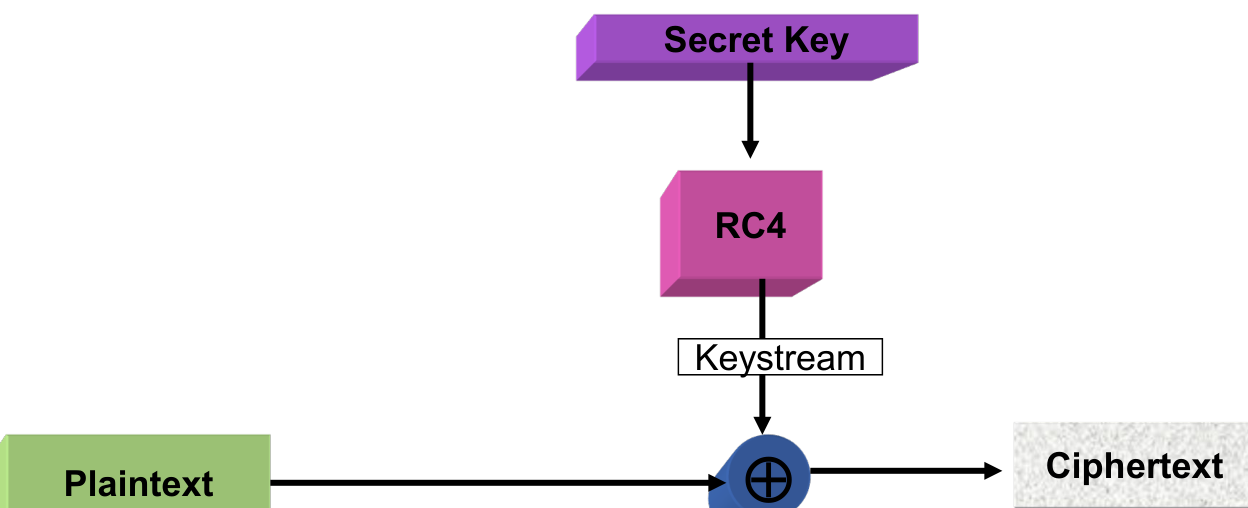
\includegraphics[width=136.50mm,height=139.59mm]{../../images/llm/page_042_img_01.png}%
\end{textblock*}

\end{document}
